\documentclass[a4paper,10pt]{article}
\usepackage[a4paper, total={7in, 9in}]{geometry}
\setlength\parindent{0pt}
\usepackage[utf8]{inputenc}
\usepackage{graphicx} 
\usepackage{amsmath}
\usepackage{amsfonts}
\usepackage{amssymb}
\usepackage{listings}
\usepackage{ragged2e}
\usepackage{listings}
\usepackage{color}
\setlength{\parskip}{\baselineskip}%
\setlength{\parindent}{0pt}%

\begin{document}
\begin{titlepage}
	\centering
	
\includegraphics[width=.6\textwidth]{liu-logo.png}\par
	\vfill
	{\scshape\Large TDDE01 MACHINE LEARNING\par}
	{\huge\bfseries Lab 3 - B18 Group Report\par}
	\vspace{0.5cm}
    {\large\itshape Lawrence Thanakumar Rajappa (lawra776)\\
     \large\itshape Grégoire Vola (grevo149)\\
     \large\itshape Kyriakos Domanos (kyrdo817)\par}
	\vfill
	{\large \today\par}
\end{titlepage}
\definecolor{dkgreen}{rgb}{0,0.6,0}
\definecolor{gray}{rgb}{0.5,0.5,0.5}
\definecolor{mauve}{rgb}{0.58,0,0.82}

\lstset{frame=tb,
  language=R,
  aboveskip=3mm,
  belowskip=3mm,
  showstringspaces=false,
  columns=flexible,
  basicstyle={\small\ttfamily},
  numbers=none,
  numberstyle=\tiny\color{gray},
  keywordstyle=\color{blue},
  commentstyle=\color{dkgreen},
  stringstyle=\color{mauve},
  breaklines=true,
  breakatwhitespace=true,
  tabsize=3
}
\textbf{\underline{Assignment - 1}} \par
The objective of this assignment is to find the temperature readings between 4 AM to 24 PM in an interval of 2 hours with independent variables
date and  place in Sweden. \par
The following data are provided as input for forecasting the temperature
\begin{itemize}
  \item \textbf{Date} : 2019-12-19
  \item \textbf{place}: \textbf{Longitude} :58.4108, \textbf{Latitude} :15.6214
\end{itemize}
The prediction is done using 3 kernels which are gaussian kernels and given below
\begin{itemize}
  \item The first to account for the distance from a station to the point of interest.
  \item The second to account for the distance between the day a temperature measurement was made and the day of interest.
  \item The third to account for the distance between the hour of the day a temperature measurement was made and the hour of interest.
\end{itemize} \par 
We use the below gaussian function for creating above-mentioned kernels,
\begin{center}
  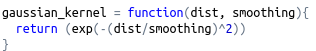
\includegraphics{gaussian_Kernel}
\end{center}
3 Smoothing coefficients are selected for the above kernels 
\begin{itemize}
  \item h\_distance = 50  \# km
  \item h\_date = 7 \# days
  \item h\_time = 3 \# hours
\end{itemize}
\textbf{\underline{Geographical Kernel}} \par
The plot below describe the weights which is provided by the 1\textsuperscript{st} kernel for each of the data points based on the distance between two places \par
\begin{center}
  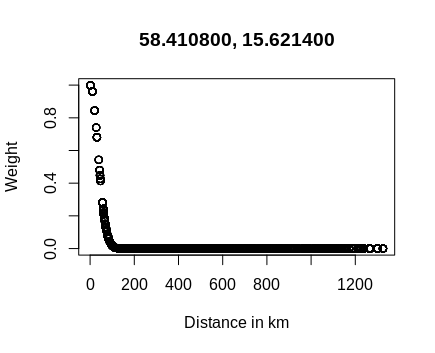
\includegraphics[width=110mm,scale=0.10]{Weights_Distance.png}
\end{center}
We can see from the above plot that as we move from the location we want to predict, the weights are getting reduced until they reach 0. This is the expected behaviour,
as one moves away from a location, the temperature calculated becomes irrelavant for the prediction. \par
\textbf{\underline{Day Kernel}} \par
The plot below describe the weights which is provided by the 2\textsuperscript{nd} kernel for each of the data points based on the difference between prediction date and
temperature measured dates (\textit{in days}).
\begin{center}
  \includegraphics[width=110mm,scale=0.10]{Weights_Day.png}
\end{center} 
From the above plot, we could see that as we move away from the date to predict, the weights are getting reduced until they reach 0. This is the expected behaviour,
as one moves away from a day, the temperature measured becomes irrelavant for the prediction.
\par
\vspace{0.5cm}
\textbf{\underline{Hour Kernel}} \par
The plot below describe the weighs which is provided by the 3\textsuperscript{rd} kernel for each of the data points based on the time difference (\textit{in hours})
\begin{center}
  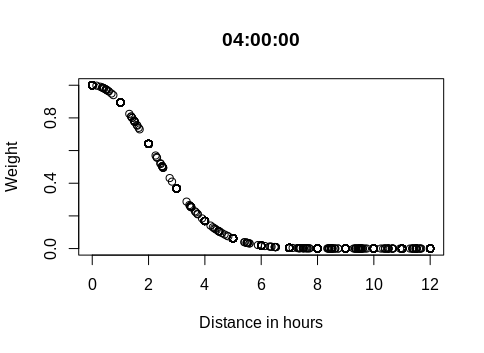
\includegraphics[width=110mm,scale=0.10]{Weights_hour.png}
\end{center}
We can see from the above plot that, as we move away from the time we need to predict, the weights are reducing until they reach 0. This is the expected behaviour,
as one moves away from a hour, the temperature measured becomes irrelvant for the prediction.
\newpage
We use the below mean function to measure the temperature,
\begin{center}
  
\includegraphics{mean.png}
\end{center} \par
\textbf{\underline{Temperature Prediction for 2019-12-19-Kernel Addition}}
\begin{center}
  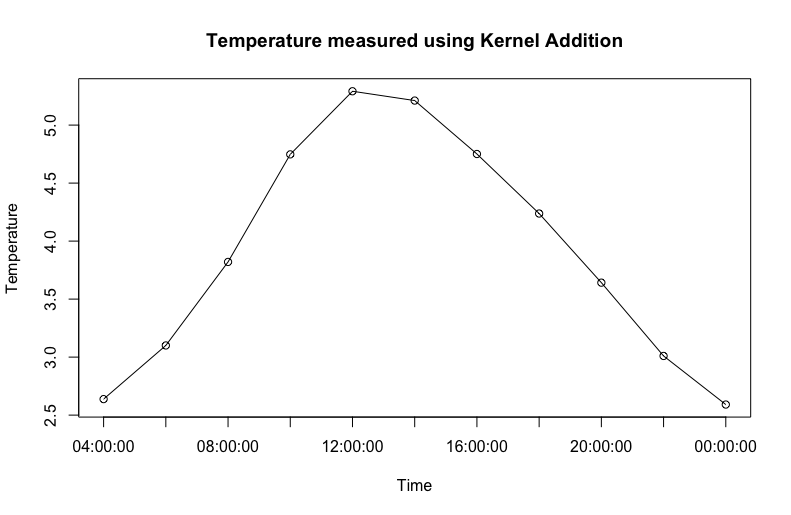
\includegraphics[width=125mm,scale=0.10]{Temp_1_Measured.png}
\end{center}
\par 
\vspace{0.5cm}
\textbf{\underline{Temperature Prediction for 2019-12-19-Kernel Multiplication}}
\begin{center}
  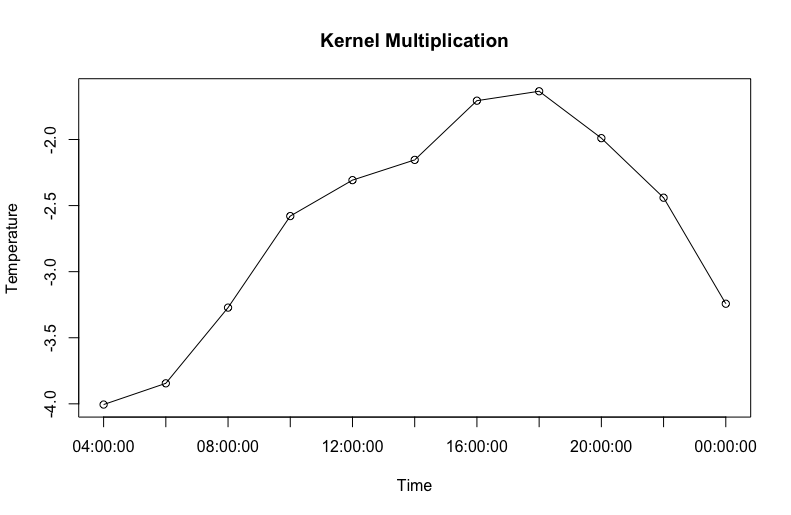
\includegraphics[width=125mm,scale=0.10]{Temp_2_Measured.png}
\end{center}
We predict the temperature by using the weighted mean of all observations temperatures. By looking the above two plots,
we can see that multiplied kernel is better than summed kernel, because summed kernel provides higher MSE error rate when
compared with multiplied kernel.
\par
\vspace{0.5cm}
\textbf{\underline{Assignment - 1 Annex}}
\par
We have performed cross-validation in order to find the best smoothing factors. please find attached code 
below for your reference. \par
\begin{center}
  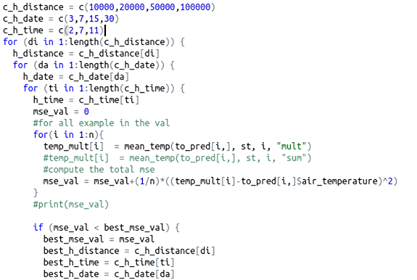
\includegraphics{Cross_Validation.png}
\end{center}
\newpage
\textbf{\underline{Assignment - 3}} \par
In this assignment, we wish to train a neural network to learn the trigonometric sine function. 
We generate uniformly 50 randoms points in the interval [0,10]. Given below is the graph of \textbf{\textit{sine}} function applied on these 50 data points \par
\begin{center}
    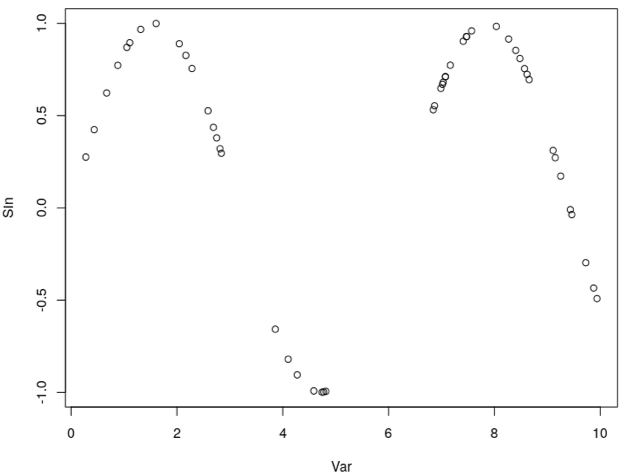
\includegraphics[width=110mm,scale=0.10]{Picture_1.png}
\end{center}
We then split the data into 2 sets: 25 points for both the training and the validation set.The training set will be used to train the neural network to learn this sine function.
The validation set will be used to detect when to stop the gradient descent in order to avoid overfitting.We are going to stop the gradient descent when the error function is below a given threshold value.
We calculate threshold by iterating 10 times i.e. \textit{i} = 1,2,3,..,10 using the below expression,
\begin{equation*}
    \frac{\textbf{\textit{i}}}{\textbf{1000}}
\end{equation*} \par
We will then choose the threshold value that minimized the error on the validation set.\par
our neural network consists of:
\begin{itemize}
    \item 1 input neuron
    \item 1 hidden layer with 10 neuron units
    \item 1 output neuron
\end{itemize} \par
We will randomly initialize all the weights of the neural network in the interval [-1,1]. 
The total weight is calculated is by,
\begin{itemize}
    \item 1 bias * 10 neurons (hidden layer)
    \item 1 intercept * 10 neurons (hidden layer)
    \item 1 bias * 1 neuron (output neuron)
    \item 10 intercept* 1 neuron (from hidden layer to output neuron)
\end{itemize} \par
We create the neural network by using the \textbf{\textit{neuralnet}} function, 
\begin{center}
    \begin{lstlisting}
        nn = neuralnet(Sin~Var,data=tr,threshold = i/1000,hidden = 10,startweights = winit)
    \end{lstlisting}
\end{center}
where,
\begin{itemize}
    \item ”Sin~Var” : we try to predict the values in the Sin column from Var column values
    \item ”data=tr”: we use tr as a training set for the NN to learn the sine function
    \item ”hidden=10”: we have one hidden layer consisting of 10 hidden neurons units
    \item ”startweights=winit”: we use the values we randomly generated to initialize the weights
\end{itemize}
We predict over the validation set and calculte the MSE for each value of the threshold. 
The threshold with the least square error is chosen as the best threshold and best neural network. \par
\begin{center}
    \begin{lstlisting}
        mse_test[i] = sum((va$Sin-pred)^2)/nrow(va) #va = validation_data
        best_Threshold = which(mse_test == min(mse_test))
    \end{lstlisting}
\end{center}
We can also select best threshold from plotting as well.After computing the error for all threshold values, 
we can plot the MSE Value of the validation data, which is given below.
\begin{center}
    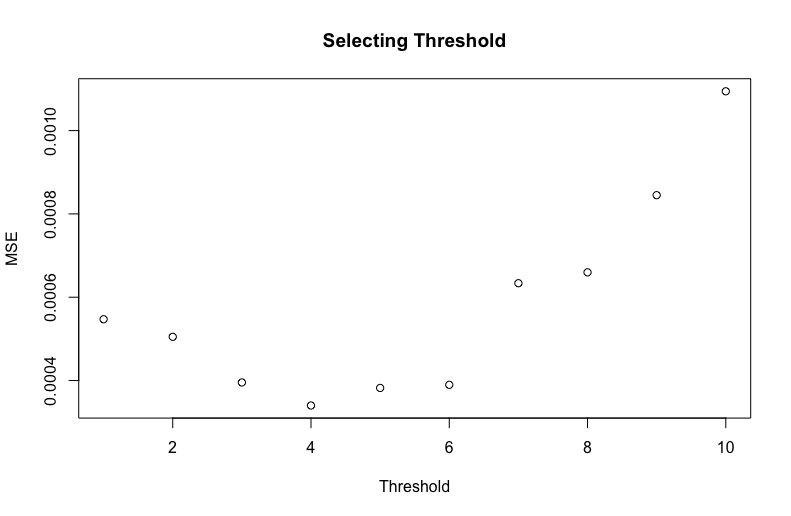
\includegraphics[width=125mm,scale=0.10]{Thresold_plot.png} 
\end{center} \par
By comparing the graph as well as value from the variable \textbf{\textit{best\_threshold}}
we chose the $threshold = 0.004$ where $i=4$.
Our minimum MSE value is \textbf{0.0003400358} \par
We plotted both the real values and predicted values which is given below,
\begin{center}
    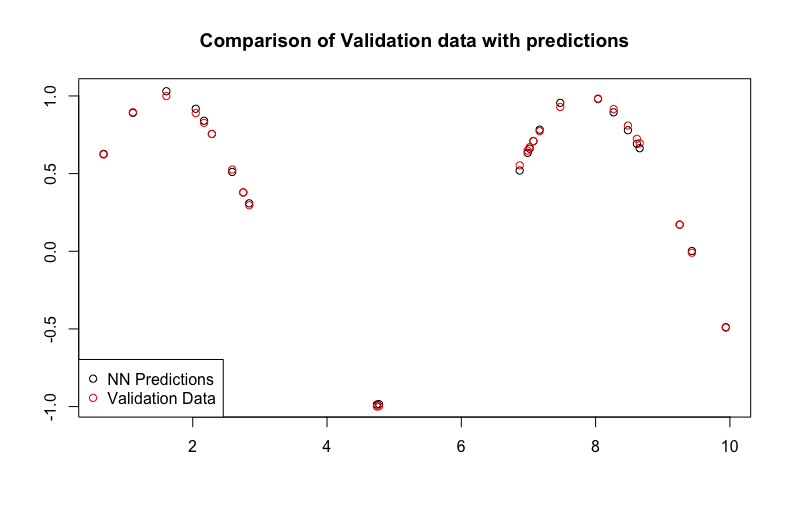
\includegraphics[width=125mm,scale=0.10]{NeuralNet_Predictions.png} 
  \end{center}
The above plot is confirming what we see from the MSE value. 
The predictions are almost perfectly matching with the real values of the sine function \par
In order to visualize the network topology with weights and biases, we are plotting the nerual network and it is given below
\begin{center}
  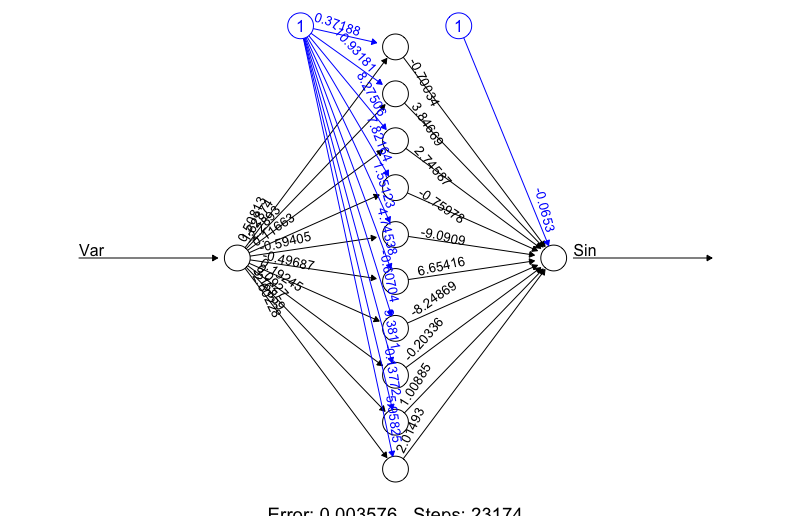
\includegraphics[width=125mm,scale=0.10]{Neural_Net_Topology.png} 
\end{center}
\newpage
\huge \textbf{\emph{\underline{Code Appendix}}} \par
\large \textit{\textbf{Assignment 1}} \par
\begin{lstlisting}
options(scipen=999) #To avoid scientific notations
RNGversion('3.5.1')

set.seed(1234567890)
library(geosphere)

get_gaussian_kernel = function(a_smoothenedDistances) {
  return(exp(-a_smoothenedDistances^2))
}

get_temp_prediction = function(a_longitude, a_latitude, a_date, a_kernelType) {

  \#Calculating geo kernel
  distanceDifference = distHaversine(c(a_longitude, a_latitude), st[4:5])/1000 #Calc in km
  geoDistance = get_gaussian_kernel((distanceDifference) / h_distance)
  plot(distanceDifference, geoDistance, main = sprintf("%f, %f",a,b), ylab = "Weight", xlab = "Distance in km")
  
  \#Calculating date kernel
  dateDifference = abs(as.numeric(difftime(st$date, a_date, units = "days")))%%365
  dateDifference[dateDifference>182] = 365 - dateDifference[dateDifference>182]
  dateDistance = get_gaussian_kernel((dateDifference)/ h_date)
  plot(dateDifference, dateDistance, main = prediction_date, ylab = "Weight", xlab = "Distance in days")

  \#Calculating time kernel
  temp_predictions = c()
  for(i in 1:length(times)) {
    timeDifference = abs(as.numeric(difftime(strptime(st$time, "%H:%M:%S"), strptime(times[i], "%H:%M:%S")), units = "hours"))
    timeDifference[timeDifference > 12] = 24 - timeDifference[timeDifference > 12]
    timeDistance = get_gaussian_kernel(timeDifference / h_time)
    plot(timeDifference, timeDistance, main = times[i], ylab = "Weight", xlab = "Distance in hours")
    
    if(identical(a_kernelType, "sum")) {
      kernel = geoDistance + dateDistance + timeDistance
    } else {
      kernel = geoDistance * dateDistance * timeDistance
    }
    temp_predictions[i] = sum(kernel * st$air_temperature) / sum(kernel)
  }
  return(temp_predictions)
}

\#Read Data
stations <- read.csv("stations.csv", fileEncoding="latin1")
temps <- read.csv("temps50k.csv")

st <- merge(stations,temps,by="station_number")

h_distance <- 50 #km # These three values are up to the students
h_date <- 7 # days
h_time <- 3 # hours

a <- 58.4108 # The point to predict (up to the students)
b <- 15.6214
prediction_date <- "2019-12-19" # The date to predict (up to the students)
times <- c("04:00:00", "06:00:00", "08:00:00", "10:00:00", "12:00:00", "14:00:00", "16:00:00", "18:00:00", "20:00:00", "22:00:00", "24:00:00")
#temp <- vector(length=length(times))

\# Students code here

\#Filter out posterior dates
st = subset(st, as.Date(st$date) < as.Date(prediction_date))

\#Prediction using kernel sum
predictionKernelSum = get_temp_prediction(a, b, prediction_date, "sum")
print(predictionKernelSum)
plot(predictionKernelSum, type="o", main = "Kernel Sum", 
     xlab = "Prediction point in temperature vector", ylab = "Temperature")

\#Prediction using kernel multiplication
predictionKernelMultiply = get_temp_prediction(a, b, prediction_date, "multiply")
print(predictionKernelMultiply)
plot(predictionKernelMultiply, type="o", main = "Kernel Multiplication", 
     xlab = "Prediction point in temperature vector", ylab = "Temperature")
\end{lstlisting} 
\par
\vspace{0.5cm}
\large \textit{\textbf{Assignment 3}} \par
\begin{lstlisting}
options(scipen=999) #To avoid scientific notations
RNGversion('3.5.1')
library(neuralnet)
library(ggplot2)

set.seed(1234567890)
Var <- runif(50, 0, 10)
trva <- data.frame(Var, Sin=sin(Var))
tr <- trva[1:25,] # Training
va <- trva[26:50,] # Validation
ggplot(trva,aes(x=Var,y=Sin))+geom_line()
# Random initialization of the weights in the interval [-1, 1]
winit <- runif(31,-1,1)
#Since we are dealing with regression, best way to choose the model is to use MSE
mse_test = rep(0,10)
mse_train = rep(0,10)

for(i in 1:10)
{
  nn = neuralnet(Sin~Var,data=tr,linear.output = TRUE,threshold = i/1000,hidden = 10,startweights = winit)
  pred = predict(nn,va)
  mse_test[i] = sum((va$Sin-pred)^2)/nrow(va)
  mse_train[i] = sum((tr$Sin-pred)^2)/nrow(tr)
}

best_Threshold = which(mse_test == min(mse_test))
plot(1:10,mse_test,xlab="Threshold",ylab = "MSE",main="Selecting Threshold")
#1st model is having lowest test error when compared with other models.
nn = neuralnet(Sin~Var,data=tr,linear.output = TRUE,threshold = best_Threshold/1000,hidden = 10,startweights = winit)

plot(prediction(nn)$rep1,col="black",xlab = "",ylab = "")
points(trva,col="red")
legend(x="top",legend = c("NN Predictions","Sin"),col=c("Black","Red"),pch = c(1,1))

plot(nn,rep="best")
\end{lstlisting}
\end{document}
